% Paper template for TAR 2020
% (C) 2014 Jan Šnajder, Goran Glavaš, Domagoj Alagić, Mladen Karan
% TakeLab, FER

\documentclass[10pt, a4paper]{article}

\usepackage{tar2020}

\usepackage[utf8]{inputenc}
\usepackage[pdftex]{graphicx}
\usepackage{booktabs}
\usepackage{amsmath}
\usepackage{amssymb}

\title{
	Search less, research more: Improving information retrieval\\
	in the face of COVID-19\\
}

\name{Mario Šaško, Ivan Lovrenčić, Nikola Buhiniček}

\address{
	University of Zagreb, Faculty of Electrical Engineering and Computing\\
	Unska 3, 10000 Zagreb, Croatia\\
	\texttt{\{mario.sasko, ivan.lovrencic, nikola.buhinicek\}@fer.hr}\\
}


\abstract{
	As the persistent COVID-19 outbreak transforms the world, scientists are vigorously researching the virus to find a cure. For researchers to stay updated with the latest developments, they have to find the time to evaluate current advancements and potentially apply them in their research. However, because of the global initiative to solve this crisis, new research is getting published continually. That causes an abundance of research papers, where most of them do not deliver any significance to the on-going cure development. To help researchers find the most prominent improvements, we propose the solution in the form of an information retrieval model, that we adapted to the scientific domain of this problem. Our model will allow researchers to find the most relevant papers for each of their COVID-19 related queries, and in the process, save some valuable time.
}

\begin{document}
	
	\maketitleabstract
	
	\section{Introduction}
	
	In the last days of 2019, numerous reports about the previously-unknown virus have appeared in Wuhan, China. Not even a few weeks after that, the World Health Organization (WHO) started alerting about a seeming global health crisis. Six months later, the highly-infectious novel Sars-Cov-2 virus has infected more than five million people and more than 340,000 people have died. Furthermore, researchers believe that this emergency will not cease until there is a viable cure, and, naturally, as a part of the global response to find it, researchers are publishing more papers than ever. However, from that arose another challenge. There is now an abundance of research papers being published, and researchers are keen to find a way to retrieve only the most prominent ones to save some precious time.

	To help researchers, the White House and the coalition of leading research groups came up with an initiative to prepare the COVID-19 Open Research Dataset (\emph{CORD-19}).\footnote{\texttt{https://www.kaggle.com/allen-institute\\-for-ai/CORD-19-research-challenge}} This accessible dataset was given to the global research community to apply various natural language processing (NLP) and machine learning (ML) techniques. These methods could help scientists find the most relevant research about the on-going pandemic and, consequently, give us a better understanding of the Sars-CoV-2 virus.

	To contribute, we have decided to develop our IR model. The main intention of our approach was to allow researchers to obtain the most relevant papers based on their query input. To achieve that, we have used a stratified model, that through each level, filters and ranks papers based on their query relevance.  The model starts with a biomedical named entity recognition (BioNER) to filter out papers that are not related to the current query. Furthermore, the model proceeds by utilizing the word (word2vec) and document (doc2vec) level embeddings to determine the remaining papers significance rank. In the end, we are left with a list of query-related papers, which are sorted based on their relevance score.

	In the following section, we will discuss the approaches of other highly-ranked proposed solutions and compare them to our own. Furthermore, in Section 3., we will explain how we used the given CORD-19 dataset for evaluation of our model, which will be explained in detail in Section 4. Moreover, in Section 5., we will talk more about evaluation and results.  We had challenges in the evaluation part, as it was hard to evaluate the significance of the research papers from the domain we are not experts. Lastly, we finish with a conclusion and ideas for future work.

	\section{Related work}

	The mentioned CORD-19 dataset came along with a series of coronavirus related tasks and so far there has been over 1,400 submissions. The task we have chosen is related to the queries about the transmission and incubation of the novel Sars-Cov-2 virus.

	In that task, the officially accepted \emph{submission}\footnote{\texttt{https://www.kaggle.com/mlconsult/\\transmission-incubation-and-environment-2-0}} is using only paper abstracts for relevance determination. Firstly, the query is being preprocessed into keywords, which are then stemmed and concatenated with COVID-19 related terms (covid, cov, -cov, hcov). Furthermore, they filter the papers by checking whether the abstract contains all of the queried keywords and at least one COVID-19 related term.

	In most of the remaining submissions, researchers calculated the relevance scores based on the keyword counts and the length of only the abstract part. However, based on our research and the impressions we encountered, the decision to use only abstracts is not justifiable and is rather wasteful. Our model utilizes more of the available data by weighting parts of papers differently, and not relying just on the short summaries.

	On the other hand, we have a highly rated probabilistic \emph{approach}\footnote{\texttt{https://www.kaggle.com/dgunning/cord-\\research-engine-search-and-similarity}}, where researchers often used a BM25 model, along with document embeddings. In those kinds of submission, they use the BM25 search index, created only from paper abstracts, as their base and boosting the performance with an Annoy index made out of 786 dimensional Specter Vectors \citep{cohan-etal-2020-specter}, which represents document embeddings. In contrast to those submissions, we have decided to utilize both word and document embeddings to get an even better insight.

	Lastly, although our model does not explicitly utilize any of the ML tools, we thought to mention one of the approaches that accomplished notable results. In the stated paper, the researchers relied more on the article body, which they parse using various NLP tools. Furthermore, they turned document into a TF-IDF based vector, on which they apply the k-means clustering. In the end, they managed to cluster papers based on some surprising factors that could potentially shed more light on this mysterious virus and the data that we have about it. However, the approach itself did not produce a state-of-the-art result.

	\section{Dataset}

	As mentioned in Section 1, we use the CORD-19 dataset to evaluate the model. The dataset contains over 134,000 scholarly articles with approximately half of them being related to COVID-19. Out of the total number, 29315 articles are presented as a full-text JSON. In the task, we focus on fields title, abstract and body and discard the rest, which aligns with our assumption that these fields are the most important ones.
	
	In order to measure the model performance, we sample the dataset and obtain 95 articles. Next, we annotated these articles as relevant or irrelevant with 3x coverage, according to the query. Finally, the majority agreement is used to define gold-standard labels.  
	
	During preprocessing, the aforementioned JSON fields are concatenated and tokenized using \emph{spaCy}\footnote{\texttt{https://spacy.io/}}, an advanced natural language processing library. Then, the input is lowercased and passed to the model. The same steps, with additional removal of stop words, are applied when working with the baselines.
	
	\begin{figure}[h]
		\centering
		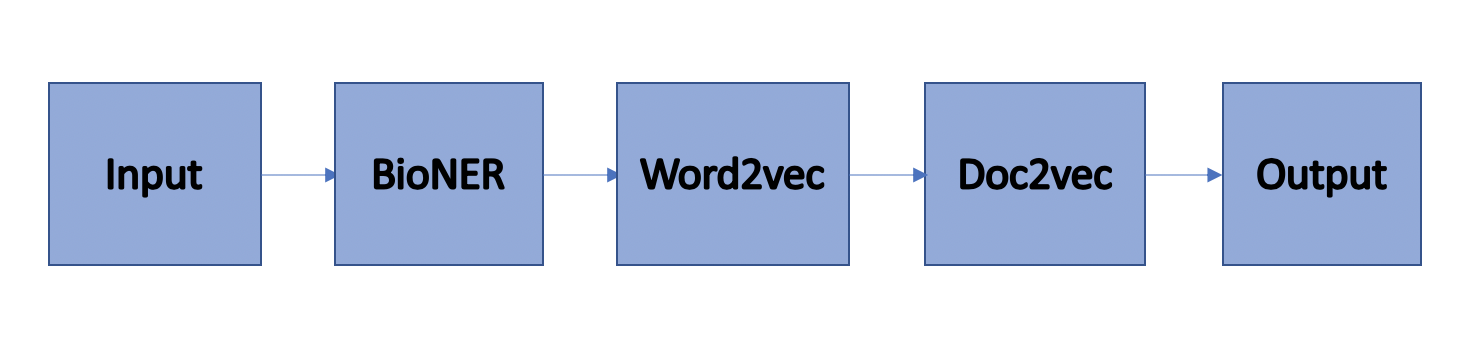
\includegraphics[width=8.5cm]{model}
		\caption{ System architecture.}
		\label{figure:model1}
	\end{figure}
	
	\section{Our approach}
	
	For our final model, we decided on a stratified structure model. We aimed to make a system where we would have the ability to add and remove layers without a lot of effort. Moreover, we wanted to have a continuous flow of data through the model, allowing us to evaluate the model at each layer. Figure~\ref{figure:model1} nicely illustrates the layered structure we have applied. 
	
	Beside distinctive system structure, our approach differs, from other submissions, in another regard. Specifically, we utilized every part of the paper, as opposed to most , where they used only the abstract. In our experiments, we have noticed that having additional data, like title or body, can make a significant difference. Consequently, we have implemented a system where each part of the paper will be treated individually. 
	
	As we can notice in Figure \ref{figure:approach}, we split our input data into three parts. Then, we pass those parts through each layer of our model. Furthermore, we sum the individual scores and calculate the average. Now, it should be noted that we repeat this process at each layer and not only at the end of the model. We use this output as the customized relevance score, which we are updating with every layer.  Lastly, the model completes with a sorted list of papers, based on the mentioned customized relevance score.
	
	In the following sections, we will explain in detail our baseline models and every individual layer in our final model. Moreover, we will describe which internal parameters we used and how we optimized them for this specific task.
	
	\begin{figure}[h]
		\centering
		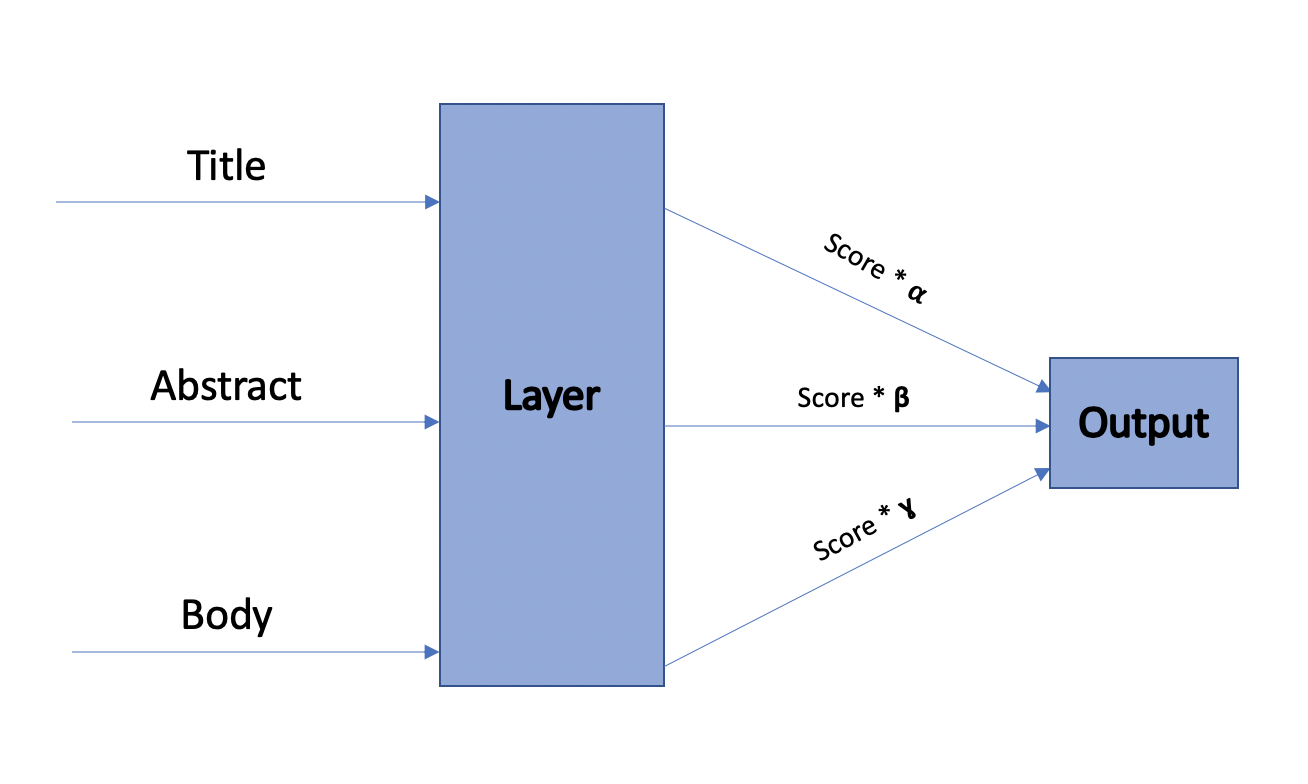
\includegraphics[width=8.5cm]{approach}
		\caption{System architecture where we score each paper based on its components.  }
		\label{figure:approach}
	\end{figure}
	
	
	\subsection{Baseline}
	
	We use two baselines to validate the performance of our model. Both models are part of \emph{Apache Lucene}\footnote{\texttt{https://lucene.apache.org/}}, a high-performance search engine library.
	
	The first one of them, an unigram Language Model (LM), builds one probabilistic model per article in collection. Then for each article, the model outputs the probability of a query belonging to it. We sort these probabilities to obtain the final relevance ranking. To make predictions more robust, the model relies on Bayesian smoothing with Dirichlet priors \citep{zhai2004study}.
	
	As our second baseline model, we use a BM25 Okapi ranking function \citep{robertson1995okapi}. The ranking function weighs query terms according to an advanced TF-IDF weighting scheme. Since this is the only function from BM family that properly scores longer articles, we don't consider other variants. Additionaly, the same sorting procedure that is used with the LM model is applied to the function output.
	
	\subsection{BioNER}
	
	BioNER is a robust NLP tool that acquires solely biomedical phrases from the given document \citep{wang2019cross}.  In our case, we applied it to extract the relevant biomedical keywords from queries and papers.  Once we obtained the keywords, we matched query keywords to the corresponding keywords from title, abstract, and body. However, we would not treat every match identically. Specifically, as we can notice from Figure \ref{figure:approach}, the final scores are multiplied with a specific hyperparameter.  Those hyperparameters were optimized specifically for this particular task, as they were used to give advantage to more significant parts of the paper.
	
	Moreover, we also applied BioNER to obtain precise keywords that should not be in the relevant papers. For example, some papers from the dataset are referring to the Sars-CoV-1, the past virus that caused an epidemic in 2003. In these situations, we want to find those phrases and appropriately correct the paper's relevance score. Without this, it was effectively impossible to differentiate between relevant and previously relevant papers, as those past papers usually include a great deal of currently relevant keywords.
	
	\subsection{Word2vec}
	
	As a complement to the previous layer, in this layer, we use word embeddings to find a semantic relation between the query and the document \cite{mikolov2013distributed}. Consequently, if the paper in the previous layer got a high score, but it is not semantically similar to the query, it will receive a low score in this layer, which will decrease its relevance score. This reiterative score recalculation allows us to find the most suitable papers, based on more than one approach.
	
	To determine the semantic similarity between them, we add each word's vector representation and then compute the cosine similarity between the query and the paper. For this part, we have applied a pre-trained Google's word embeddings. As stated, in each layer of our system, we calculate scores independently for each section of the paper - title, abstract, and body. In this case, we add up all the calculated cosine similarities, and we take an average value. 
	
	\subsection{Doc2vec}
	
In the context of the on-going pandemic, word2vec has one prominent impediment. Namely, the issue stems from the fact that most of the terminology from the current pandemic is new. Consequently, most of those new terms, like COVID-19, are not in the word2vec vocabulary, hence the overall accuracy of word2vec representations will be worse. To solve that, we added a layer of document embeddings (doc2vec). 

To build vector representations of individual papers, we have to train the doc2vec model on our dataset \cite{le2014distributed}. However, in our case, the model is exclusively trained on a subset that the prior layers listed relevant. In other words, vector representations are produced only for documents that have been named relevant by BioNER and word2vec layers. Therefore, this layer is a reinforcement layer, that will adjust the ranks, and potentially correct any irregularities in the relevance scores.

\subsection{Hyperparamters}

As previously stated, our model performance massively relies on three hyperparameters. We added those parameters because we noticed that specific sections of the paper bring much more weight than the others. 

First, we discerned that matching keywords in a title considerably increased our chances of guessing the relevant paper. However, papers that contain query words in the title are rare. Therefore, we added two more hyperparameters that would reward matched keywords in the abstract and the body. 

After numerous optimization attempts, the hyperparameters converged into the following values: $\alpha = 2.5$, $\beta = 1.5$ and $\gamma = 1$. As we can see, the title's hyperparameter has the biggest value, which implies that the title carries the most significant amount of information about the relevance of the paper. Sequentially, we see that the abstract is second and that words from the body carry the least amount of weight.


	
	\section{Results}
	
	Two COVID-19-related queries are defined to evaluate the model. For each query, the model assigns relevance scores according to which the ranking of the articles is formed. Since the resulting list contains each article from the sample dataset without the cutoff, only IR-related metrics are used. Due to the volume of the annotated data, the results are not statistically tested. 
	
	The results in Table~\ref{tab:query1} show system performance for the query \textit{What is known about Covid-19 transmission}. Reasonably high R-precision denotes that our model, as well as the baselines, is confident in the relevance of the highest-scoring articles. Furthermore, we assume that by utilizing the word and document level embeddings, the model has a chance to infer more subtle similarities between a query and an article which leads to notably higher precision at 15 and average precision. Traditional term-frequency-based approaches fail in such situations.
	
	Similarly, the results for the query \textit{What is known about Covid-19 transmission} are in Table~\ref{tab:query2}. This time our model outperforms the baselines in the ranking of 5 highest-scoring articles. Even higher average precision than in previous case signals that the model, compared to the baselines, ranks relevant articles more consistently and closer to each other.
	
	\begin{table}
		\caption{Comparison of performance for the query \textit{What is known about about Covid-19 transmission}.}
		\label{tab:query1}
		\begin{center}
			\begin{tabular}{lccccc}
				\toprule
				Model & P@5 & P@10 & P@15 & R-Prec & AveP \\
				\midrule
				LM & 0.80 & 0.60 & 0.47 & 0.67 & 0.69  \\
				BM25 & 0.80 & 0.70 & 0.47 & \textbf{0.78} & 0.70 \\
				Our Model & 0.80 & 0.70 & \textbf{0.60} & 0.67 & \textbf{0.84} \\
				\bottomrule
			\end{tabular}
		\end{center}
	\end{table}
	
	\begin{table}
		\caption{Comparison of performance for the query \textit{What is known about about Covid-19 incubation}.}
		\label{tab:query2}
		\begin{center}
			\begin{tabular}{lccccc}
				\toprule
				Model & P@5 & P@10 & P@15 & R-Prec & AveP \\
				\midrule
				LM & 0.60 & 0.50 & 0.33 & 0.60 & 0.64 \\
				BM25 & 0.40 & 0.50 & 0.33 & 0.40 & 0.55 \\
				Our Model & \textbf{0.80} & 0.50 & 0.33 & \textbf{0.80} & \textbf{0.97} \\
				\bottomrule
			\end{tabular}
		\end{center}
	\end{table}



	\section{Conclusion}

	In this paper, we presented a novel task-specific model for the query-relevance ranking of the CORD-19 articles. The model combines a biomedical named entity recognition with word- and document-level embeddings to determine the relevance score of each article. We use a LM model and a BM25 ranking function as baselines, which our model outperforms on the sample dataset.

	Note that our ultimate goal is to prove that a domain-specific model should be considered when tackling IR tasks.

	As part of future work, we would like to increase the volume of the sample dataset. This would allow us to validate our results statistically. Additionally, when annotating articles we would like to use expert knowledge and greater coverage. Lastly, the comparison with deep learning approaches would be beneficial.


\bibliographystyle{tar2020}
\bibliography{tar2020}

\end{document}
